\documentclass[11pt]{article}
\usepackage[utf8]{inputenc}\usepackage[T1]{fontenc}
\usepackage{amsmath,amssymb,amsthm}\usepackage[margin=1in]{geometry}
\usepackage{graphicx}\usepackage{booktabs}
\usepackage[hidelinks]{hyperref}
\newtheorem{theorem}{Theorem}

\title{The Prime Triplet as a Three-Member Two-Centre CRT Pattern:\\
A Non-Monotone $\omega$-Distortion on the $6N$ Skeleton}
\author{Ruqing Chen\\
\small GUT Geoservice Inc., Montreal, Quebec, Canada\\
\small \texttt{ruqing@hotmail.com}}
\date{\today}

\begin{document}
\maketitle

\begin{abstract}
Parts~IX--X showed that prime pairs straddling two consecutive centres of the $6N$
skeleton (cousins, sexy pairs) exhibit $\omega$-distortions reproduced by a
two-centre Chinese-Remainder mechanism with no fitted parameters. We extend this
from two members to three: the prime triplet $(6N-1,6N+1,6N+5)$, whose members sit
on centre $N$ (both wings) and its neighbour $N+1$ (left wing). Its dependence on
$\omega_{>3}(N)$ is \emph{non-monotone}---a rise to a peak near $\omega=3$ followed
by a fall---the signature of competing effects, twin-like enrichment on $N$ versus
the free neighbour $N+1$, exactly as for the sexy-B pair. The three-member
two-centre CRT factor, with only the wing geometry as input, reproduces this shape
on two shells: error $\le2.4\%$ for $\omega\le6$ on $S_{10}$ ($\sim2.3\times10^{6}$
triplets), with the $\omega=6$ residual tightening from $6.5\%$ ($56$ triplets on
$S_9$) to $0.5\%$ ($1832$ on $S_{10}$). The triplet is thus a three-member instance
of the same two-centre mechanism. We note that the Hardy--Littlewood triplet
constant $\mathfrak{S}(0,2,6)=2.858$ is classical; the contribution is the
non-monotone $\omega$-shape and its two-centre CRT account. No claim is made about
the infinitude of prime triplets.
\end{abstract}

\section{The triplet straddles two centres}

The only admissible triplet patterns within a span of six are $(0,2,6)$ and its
mirror $(0,4,6)$; $(0,2,4)$ is inadmissible (it occupies all residues mod $3$).
On the $6N$ skeleton, $(p,p+2,p+6)$ with $p=6N-1$ becomes
\[
  (\,6N-1,\ 6N+1,\ 6N+5\,)=(\,6N-1,\ 6N+1,\ 6(N{+}1)-1\,),
\]
so its three members occupy, as (centre-offset, wing) pairs,
$(0,-1),(0,+1),(1,-1)$: two wings on centre $N$ and one on the neighbour $N+1$.
Like the cousin and sexy pairs of Parts~IX--X, and unlike the single-centre twin,
the triplet \emph{straddles two consecutive centres}. Its $\omega$-dependence
should therefore be a two-centre distortion, not the monotone single-centre
enrichment of the twin.

\section{A non-monotone distortion}

Binning triplets by $\omega_{>3}(N)$ and normalising to $\omega=1$, the rate is
non-monotone: it rises to a peak near $\omega=3$ and then falls
(Table~\ref{tab:trip}, Fig.~\ref{fig:trip}). This is the sexy-B signature of
Part~IX: two competing effects. The twin component $(6N\pm1)$ on the conditioned
centre $N$ enriches with $\omega$ (a factor-rich $N$ protects both its wings),
while the third member on the neighbour $N+1$ behaves like the cousin's partner
(a factor-rich $N$ does not protect a wing on $N+1$), suppressing the rate at high
$\omega$. The balance produces the peak.

\section{The three-member two-centre CRT model}

We extend the Part~X factor to three members. For a prime $q>3$, with
$\mathrm{dead}(q,s)=-s\,6^{-1}\bmod q$ the residue of $N$ making the wing $6(N+
\mathrm{off})+s$ divisible by $q$, the triplet's CRT factor is
\[
  f_q=\begin{cases}
   \prod_{i}\mathbf 1\{\mathrm{off}_i\not\equiv\mathrm{dead}(q,s_i)\} & q\mid N,\\
   \dfrac{\#\{r\neq0:\ \forall i,\ r+\mathrm{off}_i\not\equiv\mathrm{dead}(q,s_i)\}}{q-1} & q\nmid N,
  \end{cases}
\]
over the three members $\{(0,-1),(0,+1),(1,-1)\}$. The rate model is
$\prod_{q\in\mathrm{POOL}}f_q$ evaluated per centre and averaged within each
$\omega$ stratum; there are no fitted parameters.

\begin{theorem}[three-member reproduction]
On $S_{10}$ ($\sim2.3\times10^{6}$ triplets), the three-member two-centre CRT
model reproduces the non-monotone $\omega$-shape to $\le2.4\%$ for $\omega\le6$.
\end{theorem}

\begin{table}[h]\centering\small
\begin{tabular}{rrcc@{\hskip 2em}rrcc}
\toprule
\multicolumn{4}{c}{$S_9$} & \multicolumn{4}{c}{$S_{10}$}\\
\cmidrule(lr){1-4}\cmidrule(lr){5-8}
$\omega$ & triplets & meas & model & $\omega$ & triplets & meas & model\\
\midrule
1 &  56114 & 1.000 & 1.000 & 1 & 356239 & 1.000 & 1.000\\
2 & 130928 & 1.034 & 1.024 & 2 & 875673 & 1.025 & 1.021\\
3 & 102726 & 1.055 & 1.039 & 3 & 768157 & 1.048 & 1.036\\
4 &  31012 & 1.020 & 1.006 & 4 & 288800 & 1.039 & 1.020\\
5 &   3071 & 0.870 & 0.852 & 5 &  43127 & 0.950 & 0.927\\
6 &     56 & 0.513 & 0.480 & 6 &   1832 & 0.691 & 0.687\\
  &        &       &       & 7 &     11 & 0.327 & 0.254\\
\bottomrule
\end{tabular}
\caption{Two-centre CRT model versus measurement, normalised to $\omega=1$. The
$\omega=6$ residual falls from $6.5\%$ ($56$ triplets, $S_9$) to $0.5\%$ ($1832$,
$S_{10}$): the $S_9$ excess was small-sample. The $\omega=7$ stratum ($11$
triplets) is too small to read; the main result rests on $\omega\le6$, where the
error is $\le2.4\%$.}
\label{tab:trip}
\end{table}

\begin{figure}[h]\centering
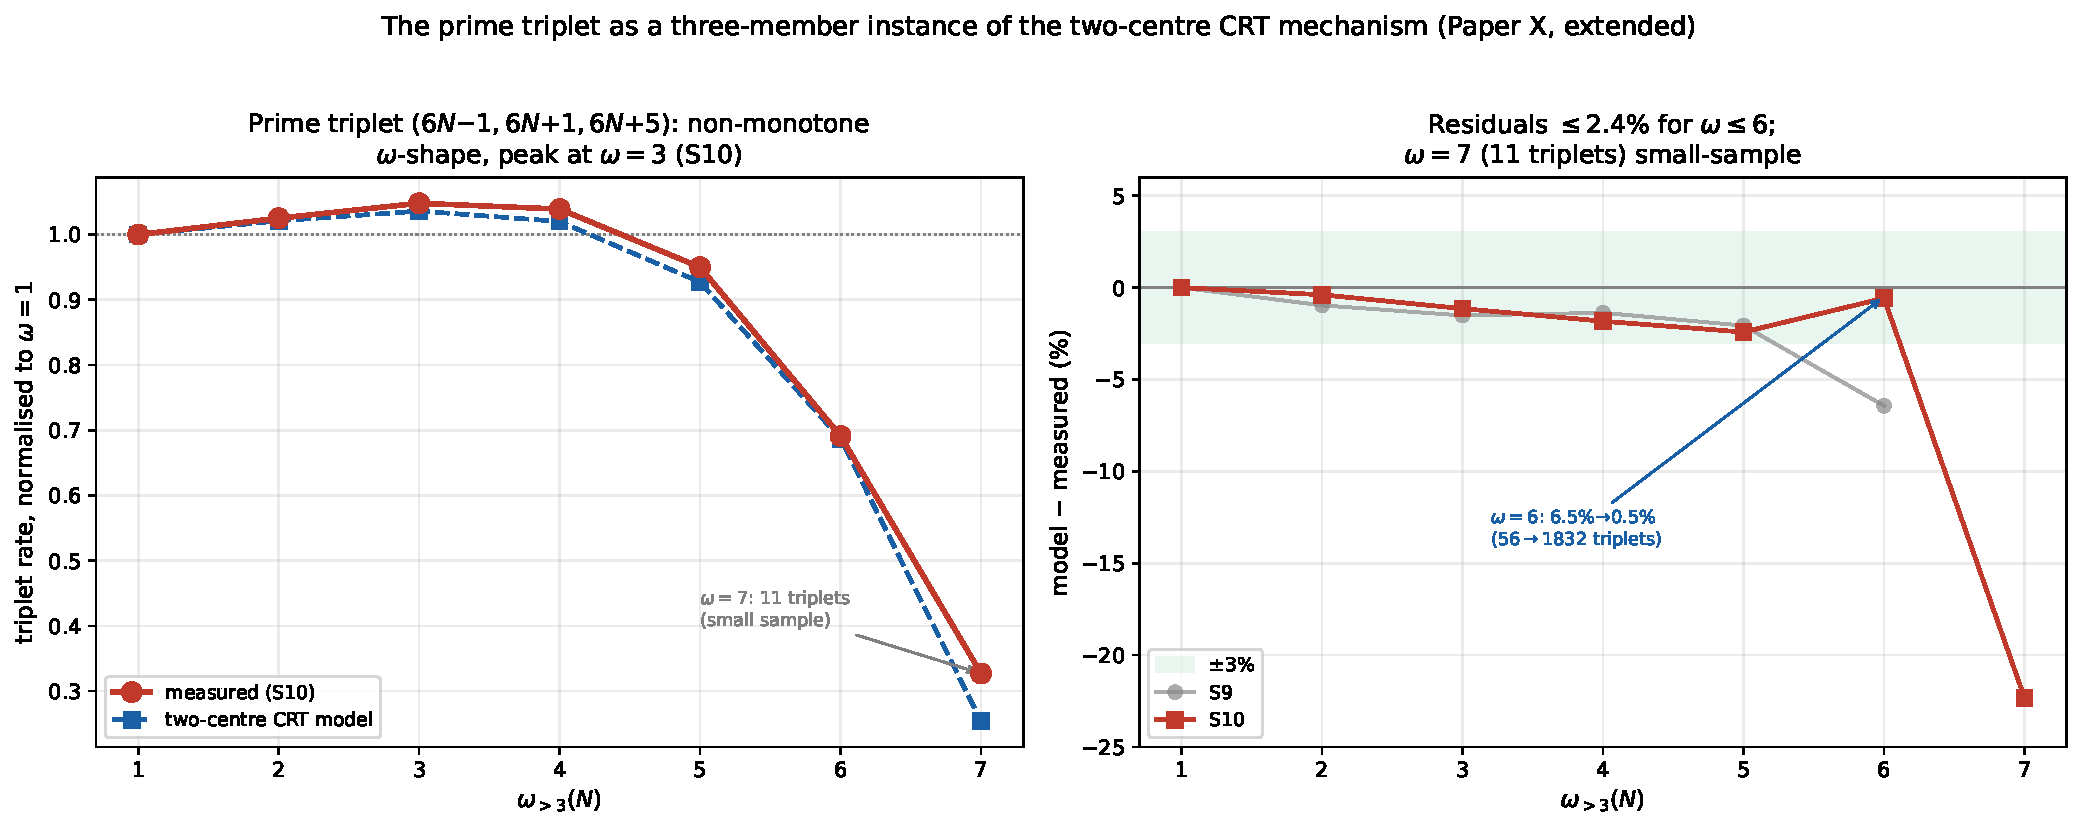
\includegraphics[width=\textwidth]{fig_paper15_triplet.pdf}
\caption{Left: the non-monotone triplet $\omega$-shape (peak at $\omega=3$), model
versus measured on $S_{10}$. Right: residuals within $\pm3\%$ for $\omega\le6$ on
both shells; the $\omega=6$ point tightens from $S_9$ to $S_{10}$ as the sample
grows; $\omega=7$ ($11$ triplets) is small-sample.}
\label{fig:trip}
\end{figure}

The decisive check on the lone large $S_9$ residual is the shell comparison: at
$\omega=6$ the error falls from $6.5\%$ to $0.5\%$ as the count grows from $56$ to
$1832$, identifying the $S_9$ excess as sampling noise. At $\omega=7$ only $11$
triplets exist on $S_{10}$; the $22\%$ residual there is not interpretable and the
result is stated for $\omega\le6$.

\section{Scope and attribution}

The triplet is a three-member instance of the two-centre mechanism of Parts~IX--X:
the same CRT factor, the same competition between the conditioned centre and its
neighbour, now with three wings instead of two, and the same non-monotone outcome
as sexy-B. The Hardy--Littlewood triplet singular series
$\mathfrak{S}(0,2,6)=2.858$ (which our sieve reproduces) is classical and sets the
overall density; this paper does not propose a new constant. The contribution is
the identification of the triplet's $\omega$-dependence as a non-monotone
two-centre distortion and its quantitative reproduction by the parameter-free CRT
model. As throughout the series, no statement is made about the infinitude of
prime triplets or any $k$-tuple conjecture; this is a measured, factor-resolved
account of the triplet's conditional rate.

\section{Conclusion}

The prime triplet $(6N-1,6N+1,6N+5)$ carries a non-monotone $\omega$-distortion---a
peak at $\omega=3$---reproduced to $\le2.4\%$ for $\omega\le6$ by the three-member
extension of the two-centre CRT mechanism, with no fitted parameters and the
$\omega=6$ residual confirmed small-sample by the $S_9\to S_{10}$ tightening. The
triplet thus joins the cousin and sexy pairs as a two-centre pattern whose
conditional shape is set by the competition between a factor-rich centre and its
free neighbour, extending the mechanism from two members to three.

\paragraph{Data and code availability.}
The triplet counts, the two-centre CRT evaluation, and the stratified statistics
are openly available~\cite{repo}.

\begin{thebibliography}{9}
\bibitem{HL} G.~H.~Hardy, J.~E.~Littlewood, \emph{Some problems of `Partitio
Numerorum'; III}, Acta Math.\ \textbf{44} (1923), 1--70.
\bibitem{ChenIX} R.~Chen, \emph{Cousin and sexy prime pairs} (Part~IX), Zenodo,
doi:10.5281/zenodo.20520492 (2026).
\bibitem{ChenX} R.~Chen, \emph{A two-centre CRT mechanism for the cousin and sexy
distortions} (Part~X), Zenodo, doi:10.5281/zenodo.20525642 (2026).
\bibitem{ChenXIV} R.~Chen, \emph{The Polignac comet under $\omega$-stratification}
(Part~XIV), Zenodo, doi:10.5281/zenodo.20533747 (2026).
\bibitem{repo} R.~Chen, \emph{$6N$ prime-triplet two-centre mechanism: data and
code}, \url{https://github.com/Ruqing1963/6N-prime-triplet} (2026).
\end{thebibliography}

\end{document}
